\documentclass[a4paper,10pt]{article}
\usepackage[top=31mm, bottom=21mm, left=16mm, right=16mm]{geometry}
\usepackage[french]{babel}
\usepackage[utf8]{inputenc}
\usepackage{textcomp}
\usepackage{url}
\usepackage{fancyhdr}
\usepackage{color}
\usepackage[colorlinks, linkcolor=black, urlcolor=black]{hyperref}
\usepackage{graphicx}
\usepackage{listings}
\usepackage{multicol}
\usepackage{sansseriftitles}
\usepackage[scaled]{helvet}
\usepackage{engord}
\usepackage{csquotes}
\usepackage[T1]{fontenc}
\usepackage[urw-garamond]{mathdesign}
\usepackage{listings}

\SetBlockEnvironment{quotation}

\setlength{\columnsep}{1cm}

\hypersetup{%
  colorlinks,
  citecolor=black,
  citebordercolor=1 0 0,
  linkcolor=black,
  urlcolor=blue,
  pdfborder=true
}

\pagestyle{fancy}
\lhead{Paul \textsc{ADENOT} \texttt{<paul@paul.cx>}}
\rhead{Département informatique, année 2011/2012}
\cfoot{\thepage}
\setlength{\parskip}{1em}
\setlength{\headheight}{13.6pt}

\newcommand{\cc}[1]{\texttt{#1}}
\title{\textsf{\textbf{Rapport de Synthèse\\Implémentation de nouvelles
fonctionnalités media dans Gecko}}}
\author{Paul \textsc{Adenot}, \texttt{<paul@paul.cx>}}
\date{}

\begin{document}
\maketitle
\subsection*{Entreprise d'accueil:}
\noindent
Mozilla Corporation\\
650 Castro Street\\
Suite 300\\
Mountain View, CA, 94041-2021\\
USA\\

\subsection*{Enseignant responsable:}
\noindent
Előd \textsc{Egyed-Zsigmond}

\section*{Résumé}
La fondation Mozilla est une organisation à but non lucratif qui a pour but de
promouvoir un Web ouvert à tous, par l'intermédiaire de son produit phare,
le navigateur web Firefox. Durant ce stage, de nouvelles fonctionnalités dans
le composant media du logiciel ont été implémentés, ainsi que des optimisation
de la vitesse de rendu des documents. Il sera aussi évoqué les processus
particuliers de travail que l'entreprise a adopté, ainsi que ses relation avec
les organismes de standardisation des normes qui font le web, de nos jour.

\section*{Mots-clefs}
Mozilla, logiciel libre, media, thread, codec, travail distribué,
réechantillonage, time-stretching, type MIME, media query, box blur, dégradé,
spécification, Web.
\section*{Abstract}
The Mozilla Foundation is a non-profit organization whose goal is to promote a
open Web, by creating and maintaining its main product, the Firefox web browser.
During this internship, new features of the media component of Firefox have been
implemented, along with a few optimizations of the rendering speed of documents.
There will be mention of the particular processes the organization had to adopt,
and its relation to the organizations that write the specifications for the web
technologies.

\section*{Keywords}
Mozilla, free software, media, thread, codec, remote working, resampling,
time-stretching, MIME type, media query, box blur, gradient, specification, web.

{\footnotesize
\tableofcontents
}

\clearpage

\begin{multicols}{2}
  \part*{Introduction}
  J'ai effectué mon stage de fin d'études au sein de l'entreprise Mozilla
  Coporation, filliale de la Mozilla Foundation, bien connue pour son navigateur
  Mozilla Firefox.

  Mozilla Firefox est un des navigateurs web les plus utilisés (entre 20\% et 50\%
  des parts de marchés, selon les pays). De plus, il est le seul contrôlé par
  une organisation à but non-lucratif, ce qui le distingue de ses concurrents.

  L'arrivée du nouveau standard HTML5\cite{HTML} a introduit les balises \cc{<audio>}
  et \cc{<video>} parmi les nouveaux éléments disponible pour rédiger des pages
  dans le langage HTML5. Les auteurs de site web commençant à utiliser
  ces balises de plus en plus, il est donc nécessaire au éditeurs de navigateur
  d'implémenter la spécification, pour rester compétitif.

  Ce stage a principalement consisté à implémenter quelque fonctionnalités de
  de cette spécification, mais aussi à discuter de la pertinence de cette
  spécification, lorsqu'elle ne paraissait pas tout a fait adéquat.

  Vers la fin du stage, les tâches qui m'avaient été assignées étant terminées,
  et voulant découvrir une autre partie du code de Firefox, j'ai commencé, sur
  une suggestion de mon manager, a écrire du code dans le sous-système
  \cc{layout} et rendu graphique.

  Nous commencerons par une bref introduction a l'architecture logicielle de
  Firefox, puis nous nous concentrerons sur le sous-système media. Nous
  passerons en revue certaines des fonctionnalités implémentés, en détaillant
  les points intéressant de chacune, pour finir sur un bilan des processus
  utilisés pour travailler au sein du projet.

  \part{Contexte}
  \section{Vue d'ensemble du sous-sytème media}
  La plus grande partie du stage à été passé dans cette partie du code, que l'on
  retrouve dans les dossiers \cc{content/media}, \cc{content/html/content/} et
  \cc{media/} de \cc{mozilla-central}, le dépot dans lequel se trouve le code
  source pour Firefox. En plus des fonctionnalités présentés dans la seconde
  partie, bon nombre d'autre patches ont été écris, parce qu'il corrigeaient un
  bug qui \og bloquait \fg un autre patch, ou encore pour ajouter des
  fonctionnalités qui étaient d'un moins grand intérêt pour ce rapport.

  L'arrivée de la lecture de media dans Gecko date de 2009, avec la sortie de
  Firefox 3.5. Cette partie du code est est relativement complexe, puisque
  complètement asynchrone. Ce choix technique est nécessaire, puisque les
  différentes partie de la lecture d'un média (qu'il soit audio ou vidéo)
  peuvent provoquer des opérations bloquantes. Il est bien entendu inacceptable
  de bloquer le thread principal de l'application (qui rend l'interface
  graphique et gère les interactions utilisateurs) lorsque le décodeur WebM est
  en train de lire dans la socket ou dans le cache disque une vidéo pour la
  décoder. De la même manière, il serait malheureux d'avoir des pauses dans la
  lecture d'une chanson parce que le thread principal est surchargé (par
  exemple, en train d'exécuter du code Javascript).

  Cela rend le code assez complexe a la lecture: là où pour du code synchrone,
  il suffit de lire linéairement, il faudra garder plusieurs états et sauter de
  fonction en fonction et de fichier en fichier pour comprendre du code
  asynchrone.

  Le \cc{nsHTMLMediaElement} est la classe qui gère les éléments \cc{<audio>} et
  \cc{<video>} dans Gecko. Elle fonctionne sur le thread principal et gère
  l'interaction avec Javascript.

  Le \cc{nsBuiltinDecoder} contient un cliché, a un instant $t$ du décodeur
  sous-jacent, disponible sur le thread principal.  Les décodeurs n'étant pas
  sur le thread principal, cela permet à du code Javascript et à l'interface
  utilisateur d'avoir de nouvelles informations sans bloquer.

  La classes \cc{nsBuiltinDecoderStateMachine} orchestre la décompression des
  media, la machine à états pour la lecture, l'envoie de buffer audio vers du
  code spécifique à chaque plateforme pour la lecture (\emph{platform audio
  backend}), l'enfilage des images des vidéo dans des \emph{media queues}, la
  synchronisation audio/video, et la logique de \cc{buffering}. Cette classe
  fonctionne sur un thread partagé par toutes les instances d'éléments
  \cc{<audio>} et \cc{<video>}.

  Les classes \cc{ns*Reader} implémentent la glue avec les bibliothèques
  spécifiques de décompression (\cc{libvorbis}, \cc{libtheora}, \cc{libvpx},
  etc.). Si l'on veut que Gecko puisse lire un nouveau codec, il suffirat donc
  d'implémenter une nouvelle classe de type \cc{ns*Reader}, et d'ajouter quelque
  ligne à d'autre endroit du module.

  La classe \cc{nsAudioStream} gère la lecture audio. Elle encapsule deux
  bibliothèques, \cc{libsydneyaudio} et \cc{libcubeb}, qui permettent toutes
  deux de jouer du son de manière multi-plateforme (Windows, MacOS, Linux
  Pulseaudio et ALSA, Android, *BSD, Boot to Gecko). Gecko est actuellement en
  train d'effectuer la transition de la première bibliothèque a la seconde.

  La classe \cc{MediaResource} abstrait le mode de transport du fichier, et
  fourni la même API a l'utilisateur, que le fichier provienne du disque dur,
  d'un site internet, ou du cache disque. C'est là que se fait l'intégration
  avec la pile réseau du navigateur.

  La classe \cc{nsMediaCache} gère un cache disque, de taille fixe, qui permet
  de rejouer un média sans avoir besoin de faire appel au réseau. Le cache est
  détruit lors de la fermeture de Firefox, et la clé pour chaque entrée est
  l'URL du média.

  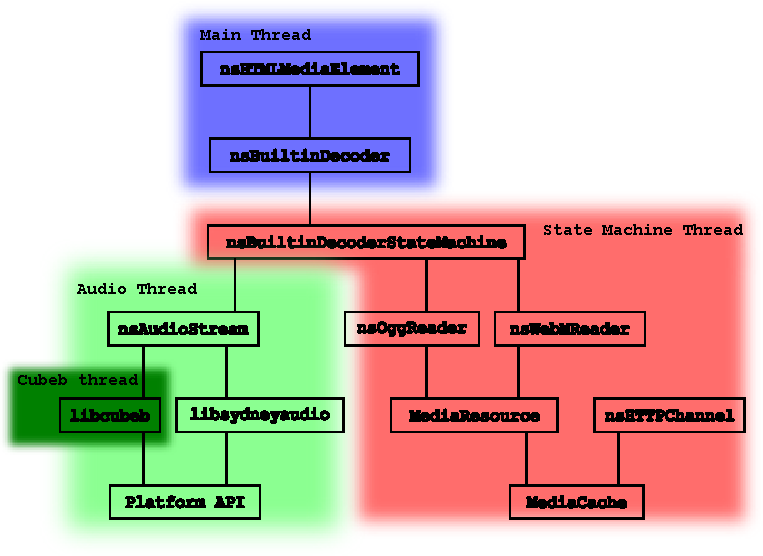
\includegraphics[width=0.40\textwidth]{img/content-media.pdf}

  \part{Synthèse technique}
  \section{Proprieté \cc{playbackRate} des éléments \cc{<audio>} et \cc{<video>}}
  Une des propriétés des éléments media que spécifie HTML5 est de pouvoir en
  changer la vitesse de lecture. Cela se fait au travers de la propriété
  \cc{playbackRate}, accessible en Javascript dans une page web. Comme son nom
  l'indique, si un auteur assigne la valeur 0.5 a cet attribut, le media devrait
  jouer deux fois plus lentement, et deux fois plus rapidement si a l'inverse il
  lui affecte la valeur 2.0.

  Changer la vitesse de lecteur d'une vidéo qui n'a pas de piste audio n'est pas
  très compliqué: il suffit de changer la vitesse a laquelle on donne des
  nouvelles images depuis le décodeur au moteur de rendu, en prenant bien garde
  a en informer tous les composants: horloge media, compensée avec la vitesse de
  lecture, logique de téléchargement et de décodage, pour éviter de se retrouver
  avec un surplus ou manque d'images a afficher.

  Par contre, tout se complique lorsque le média dispose d'une piste audio. Il
  faut alors effectuer une étape de rééchantillonnage (\emph{resampling}). Ce
  procédé permet changer, comme son nom l'indique, la fréquence
  d'échantillonnage d'une piste audio numérisée. Si l'on double la fréquence
  d'échantillonnage (par exemple de 48000Hz vers 96000Hz), mais que l'on continue
  a jouer le media a 44100Hz, on aura donc un ralentissement d'un facteur deux.

  Le composant de rééchantillonnage du codec voix Speex a été utilisé dans un
  premier temps pour effectuer cette tâche. Cependant, on observe qu'une
  division par deux en fréquence d'échantillonnage a pour effet de bord de
  transposer la piste audio une octave plus grave. Une seconde bibliothèque,
  SoundTouch, a été utilisé a la place pour profiter d'un effet appelé
  \emph{time-stretching}, qui consiste a change la vitesse d'une piste audio,
  sans en changer la hauteur.

  Ces deux bibliothèques, de licence compatibles avec celle de Firefox, et
  multi-plateforme, ont été intégré dans le dépôt principal du projet
  (\cc{mozilla-central}).

  La principale difficulté dans cette fonctionnalité aura été qu'elle nécessite
  des modification a tous les niveaux du sous-sytème media. De plus, une grande
  partie du temps a été utilisé pour trouver la bonne manière de permettre à
  l'utilisateur de changer la vitesse de lecture de manière dynamique lorsque le
  média est en train de jouer. Cela a nécessité la mise en place de mécanisme de
  compensation de latence relativement complexe.

  \section{Attribut \cc{media} de la balise \cc{<source>}}

  Les balises \cc{<source>}, placées a l'interieur d'une balise \cc{<audio>} ou
  \cc{<video>}, permettent de spécifier différent média disponible, que le
  navigateur pourra choisir, en fonction des codec, mais aussi de la résolution
  de ce qu'on appelle une \emph{media query}, avec l'attribut \cc{media} implémenté
  durant ce stage.

  Une \emph{media query} est une expression s'évaluant en un booléen, qui permet
  normalement de restreindre certaines règles CSS a un certain type de media
  (ici, au sens de \emph{support}):

  \noindent
  {\footnotesize
  \cc{/* Cette portion de la feuille de style s'applique\\
     à des périphériques ayant une largeur de plus de 500px */\\
     @media (min-width:500px) { color: red; }\\
     /* Cette portion s'applique lorsque l'utilisateur tient\\
     son périphérique en mode portait: */ \\
     @media (orientation:portrait) { width: 80\%; }
  }}

  L'idée est donc de pouvoir sélectionner une certaine \cc{<source>} en fonction
  du type d'appareil que l'utilisateur utilise pour rendre un certain media. En
  effet, visionner une vidéo 1080p sur une smartphone vertical disposant d'une
  largeur de 500 pixels est un gâchis de bande passante, et de batterie, puisque
  le périphérique doit d'abord décoder une vidéo haute définition, puis ensuite
  la ré-échantillonner pour l'adapter a la taille de l'écran, ce qui augmente
  grandement les calculs a faire, et donc la consommation d'énergie. La première
  source qui a une \emph{media query} évaluée à vrai (ou qui n'a pas de \emph{media
  query}) sera sélectionnée, sous réserve que le navigateur puisse décoder le
  codec dans laquelle il est encodé.

  \noindent
  {\footnotesize
    \cc{%
      <video controls preload=metadata>\\
      <source src="lapin-sd.webm" media="max-width: 500px">\\
      <source src="lapin-hd.webm">\\
      <source src="lapin-sd.mp4" media="max-width: 500px">\\
      <source src="lapin-hd.mp4">\\
      </video>\\
    }
  }

  La majorité du code (parseur et résolveur de règle \cc{media}) est en fait
  appelé directement depuis le code qui gère le CSS.

  \section{Détection de type MIME par reniflage}
    Les types MIME (Multipurpose Internet Mail Extensions), étaient à l'origine
    est type spécifiant le type des contenu envoyés par email. De nos jours, ils
    sont envoyés avec la réponse à une requête HTTP pour indiquer le type selon
    lequel le navigateur devra interpréter la ressource. Par exemple, une page
    HTML classique est de type \cc{text/html} et une feuille de style CSS
    \cc{text/css}. Dans Gecko, et plus particulièrement dans le code des balises
    media, ces types MIME sont utilisés pour savoir quel décodeur instancier, en
    fonction du type du fichier. Gecko supporte les types suivants:

    \begin{itemize}
      \item \cc{audio/ogg}, \cc{video/ogg} pour les contenus audio et video
        encapsulés dans un conteneur OGG contenant du Vorbis, Theora ou Opus.
      \item \cc{audio/webm} ou \cc{video/webm} pour les contenus audio et video
        encapsulés dans un conteneur WebM, contenant du VP8 et du Vorbis.
      \item \cc{audio/wav} pour un fichier audio Wave, qui est en faite les
        donnés audio non compressées.
      \item \cc{video/mp4} pour un fichier dans un conteneur mp4, contenant du
        H.264 et de l'AAC (uniquement si certaines option de compilation sont
        activées, puisque ces codecs ne sont pas libres).
    \end{itemize}

    Si le type MIME n'est envoyé dans les en-têtes de la réponse à la requête
    HTTP envoyée par le navigateur, ou s'il est erroné, le media ne pourra pas
    être décodé correctement, et par conséquent ne pourra pas être lu par ne
    navigateur. Certain très gros service d'hébergement de donnée (Amazon S3,
    par exemple) n'envoyaient pas, pendant un temps, ce type MIME, rendant 
    illisible les media provenant de ce fournisseur dans Firefox.

    La solution, en plus de communiquer sur la nécessité d'envoyer un MIME type
    correct avec une réponse HTTP, est de tenter de determiner le type du
    fichier en regardant son contenu, après en avoir téléchargé le début. Cette
    technique est appelée \emph{binary sniffing}.

    Techniquement, il aura fallu créer un composant capable d'être appellé par
    la couche réseau de Firefox (appelée \cc{necko}, et située dans le dossier
    \cc{netwert} (sic)), et à qui est envoyé les 512 premier octets du fichier,
    si le type MIME n'est pas connu.

    On applique a ces 512 premier octets un traitement  (souvent à base de ET
    binaire et de masque), pour déterminer son type. Ainsi, on obtient la table
    suivante:

    \begin{center}
      \begin{tabular}{ l | c | r }%
        Premiers octets & Masque                          & Type \\ \hline
             \cc{OggS0} & \cc{0xffffffff}                 & Ogg  \\
      \cc{RIFF0000WAVE} & \cc{0xffffffff00000000ffffffff} & Wave \\
        \cc{0x1a45dfa3} & \cc{0xffffffff}                 & WebM \\
            \cc{0xfffa} & \cc{0xfffb}                     & MP3  \\
               \cc{ID3} & \cc{0xffffff}                   & MP3  \\
      \end{tabular}
    \end{center}

    En masquant les $n$ premiers octets du fichier avec le masque et en les
    comparant avec ceux spécifiés, il est donc possible de déterminer le type du
    média, d'instancier le bon décodeur, et donc de pouvoir présenter le média à
    l'utilisateur. Cette technique est spécifié dans un document du WhatWG
    \cite{Sniff}. L'implémentation de Gecko prend en charge plus de type de
    média que la spécification, qu'il faudra probablement mettre à jour pour
    refléter les nouveaux type de fichier lisible dans les navigateurs.

  \section{Mise en cache du dessin des dégradés}

  Lorsqu'un développeur web veut dessiner un dégradé dans une page HTML, il doit
  le spécifier en CSS en utilisant une syntaxe particulière:

    \noindent
  {\footnotesize
  \cc{/* Dégradé linéaire a 45 degrés du bleu au rouge. */\\
    background: linear-gradient( 45deg, blue, red );\\
    /* Un dégradé d'en bas à droite en haut à gauche,\\
       du bleu au rouge. */\\
    linear-gradient(to left top, blue, red);\\
  }}

  Lorsque le moteur de rendu voit une de ces règle, il doit calculer le dégradé
  qui devra être affiché, en fonction des différents \emph{stops}, direction et
  couleurs, et de la taille du dégradé lui même. Ce calcul (principalement des
  calculs d'interpolation) est re-effectué à chaque fois que le dégradé devra
  être affiché par le navigateur. Cependant, remarque assez rapidement que le
  résultat de ce calcul pourrait être stocké et réutilisé: le dégradé d'un
  onglet de Firefox ne devrait pas être recalculé tout le temps: il est le même
  pour tout la durée de vie de l'application. De même, les dégradés revenant
  souvent dans une page Web devraient être cachés.

  Dans Gecko, les dégradés sont rendus par Cairo, bibliothèque de dessin
  multi-plateforme, qui abstrait les opérations de dessin à des solutions
  spécifiques a la plateforme: GDI+ (logiciel) ou Direct2D (accéléré
  matériellement) sur Windows, Quartz sur MacOS, Xlib pour Linux, GL, etc.

  Lorsque le dessin est fait de manière logicielle, par le CPU, le temps pour
  peindre la surface est vraiment plus important que le temps utilisé pour
  calculer les dégradés. Cependant, avec l'arrivée dans les navigateurs de
  l'accélération matérielle, une opération de ce type prend tout son sens: le
  dessin du dégradé est fait par le GPU, ce qui fait que le calcul du dégradé
  devient l'opération la plus longue.

  Techniquement, il aura suffit d'avoir une table de hachage, avec la
  spécification du dégradé et sa taille en clée, et le résultat du calcul en
  valeur. La politique d'éviction du cache est basé sur la durée: si telle
  entrée n'a pas été utilisé depuis $n$ secondes, on retire l'élément du cache.

  Trouver une bonne valeur pour $n$ a été fait de manière empirique. On utilise
  pour cela le composant \emph{Telemetry} de Firefox, permettant, sur accord de
  l'utilisateur, de renvoyer a Mozilla des données anonymisées.

  En donnant a $n$ une valeur aléatoire, et en mesurant le temps de rendu des
  dégradé, tout en renvoyant ces deux valeurs, il sera possible de déterminer
  une bonne valeur pour ce $n$. Ceci est un projet en cours, et était catégorisé
  au plus haut degré de priorité dans le projet Snappy, visant à améliorer les
  performances de Firefox.

  \section{Optimisation des routines de flou pour dessiner les ombres}

  Une autre propriété apparue assez récemment dans les navigateurs est la
  possibilité de spécifier un flou sur du texte ou une boite (\cc{<div>},
  \cc{<span>}, etc.). En CSS, on spécifie une ombre de la manière suivante:

    \noindent
  {\footnotesize
  \cc{/* Text avec une ombre noire décalé de 4px\\
    en abscisse par 4px en ordonnée, avec 2px de flou. */\\
    text-shadow: 4px 4px 2px black;\\
    /* Boite avec une ombre rouge de 2px par 3px\\
    avec un flou de 4px. */\\
    box-shadow: 2px 3px 4px rgba(255, 0, 0, 1.0);
  }}

  Une ombre se dessine en deux partie: premièrement, on copie l'objet et on le
  décale de la distance spécifiée, puis on le floute. La première partie de
  résume à faire un appel à la fonction \cc{memcpy}. La seconde est plus
  technique. Le standard dit:

  \begin{quote}
    A non-zero blur distance indicates that the resulting shadow should be
    blurred, such as by a Gaussian filter. The exact algorithm is not defined;
    however the resulting shadow must approximate (with each pixel being within
    5\% of its expected value) the image that would be generated by applying to
    the shadow a Gaussian blur with a standard deviation equal to half the blur
    radius.
  \end{quote}

  Le standard donne donc au concepteurs de moteurs de rendu une certaine
  latitude quant à la technique à utiliser pour calculer le flou, tant qu'elle
  est de qualité suffisante. En pratique, si on lit le code des moteurs de rendu
  open-source (Gecko, Webkit), un algorithme appelé \emph{box blur} est utilisé.
  Il approxime a 3\% près une flou gaussien, tout en permettant de travailler en
  deux passes verticales et horizontales.

  L'implémentation de Gecko était trop lente: le défilement de pages contenant
  beaucoup d'ombres était saccadé sur des machines même relativement récentes.
  En extrayant l'algorithme de Gecko et en l'analysant a l'aide d'outils de
  \emph{profiling} tels que \cc{valgrind} (simulateur de CPU x86),
  \cc{cachegrind} (analyseur permettant de déterminer le taux de défaut de
  cache) et \cc{gprof} pour un mesure de performance plus classique. Cela a
  permis de localiser les points faibles de l'algorithme, et d'en réécrire une
  version environ deux fois plus rapide, en étudiant les accès mémoires
  nécessaires, et les optimisation que peuvent faire les compilateurs. Une
  méthode de mesure de performance basée sur des données quantitative a été mise
  en place, ce qui a permis de justifier certains choix pas forcements évidents,
  mais qui, du fait des optimisations que peuvent faire les processeur récent
  x86 et ARM (cache line prefetching, stride prediction, write-combining, prise
  en compte du pipelining, etc.), résultaient en de meilleurs performances.

  D'autre optimisations seront possibles dans le future: utilisation de SSE et
  de NEON, jeu d'instruction vectoriels sur x86 et ARM, mise en cache des
  dessins des flous, copie de zone du flou au lieu d'effectuer un recalcul
  (lorsqu'on remarque que lors d'un \cc{box-shadow}, la plupart des lignes et
  des colonnes peuvent n'être calculés qu'une fois puis copiés).

  \part{Synthèse au niveau processus}
  \section{Vie d'une fonctionnalité dans Gecko}
  \section{Environnement de travail}
  \part{Bilan}

\bibliographystyle{abstract}
\bibliography{PaulADENOT-Report.bib}

\end{multicols}

\end{document}

